% TeX root = main.tex

% First argument to \section is the title that will go in the table of contents. Second argument is the title that will be printed on the page.
\section[Lecture 1--{Riemannian manifold}]{1. Riemannian manifold}

\subsection{Inner Products on a Vector Space}
The $\textbf{Euclidean inner product}$ on $\mathbb{R}^n$ is defined by
\begin{align}
    \inner{u}{v}=\sum_{1}^{n}u^i v^i,
\end{align}
and the length of a vector is
\begin{align}
    \norm{u}=\sqrt{\inner{u}{u}},
\end{align}
the \textbf{angle} $\boldsymbol{\theta}$ between two vectors is
\begin{align}
    \cos \theta = \frac{\inner{u}{v}}{\norm{u}\norm{v}},
\end{align}
the \textbf{arc length} of a curve $c(t) \in \mathbb{R}^n, a \leq t \leq b$ is 
\begin{align}
    s = \int_{a}^{b} \norm{c'(t)} dt
\end{align}

\begin{definition}
    An inner product in a real vector space $V$ is a postive-definite,
    bilinear and symmetric map: $\inner{\cdot}{\cdot}: 
    V \times V \rightarrow \mathbb{R}$ 
    so that for $u,v,w \in V$ and $a,b\in \mathbb{R}$, satisfies
    \begin{enumerate}[label= (\roman*)]
        \item \textbf{Postive-definiteness} $\inner{v}{v}=0$ iff. $v=0$
        \item \textbf{Symmetry} $\inner{u}{v}=\inner{v}{u}$
        \item \textbf{Bilinear} $\inner{au+bv}{w}=a\inner{u}{w}+b\inner{v}{w}$
    \end{enumerate}
\label{def. inner prodcut}
\end{definition}

\begin{proposition}
    If $W$ is a subspace of $V$, then the restriction
    \begin{align}
        \inner{}{}_W:=\inner{}{}|_{W\times W}: W \times W \rightarrow \mathbb{R},
    \end{align}
    of an inner product
    $\inner{}{}$ on $V$ is also an innver prodcut.
\end{proposition}
\begin{proof}
    The subspace construction preserves the properites 
    in Definition~\ref{def. inner prodcut}.
\end{proof}

\begin{proposition}
    The \textbf{nonnegative linear combinition} of inner products $\inner{}{}_i$
     on $V$: $\inner{}{}:=\sum_{i=1}^{r}a_i\inner{}{}_i, a_i \geq 0$ is again an 
     inner product on $V$.
\label{prop. nonneg combinition of metrics}
\end{proposition}
\begin{proof}
    The \textbf{nonnegativity} of $a_i$ preserves condition $(i)$ 
    in Definition~\ref{def. inner prodcut}, the linearity makes condition $(ii),(iii)$ hold.
\end{proof}

\subsection{Representations of Inner Products by Symmetric Matrices}
Let $e_1,\dots, e_n$ be the basis of vector space $V$, 
each vector $x \in V$ can be represented as a column vector
\begin{equation}
    x=\sum_{i=1}^{n}x^i e_i \leftrightarrow \vx=\left[\begin{array}{c}
        x^1 \\
        \vdots \\
        x^n
    \end{array}\right].
\end{equation}
Let $\mA$ be an $n\times n$ matrix whose entries $a_{ij}=\inner{e_i}{e_j}$, 
the matrix form of an inner product on $V$ is
\begin{equation}
    \inner{x}{y}=\sum_{ij}x^i y^j \inner{e_i}{e_j} = \vx^\top \mA \vy.
\end{equation}
We find that, once a basis of $V$ is chosen, the inner product on $V$
determines a postive-definite symmetric matrix. Conversely, an $n \times n$
postive-definite symmetric matrix with a basis of $V$ determines an inner product 
on $V$

It follows that there is an one-to-one correspondence
\begin{align}
    \left\{
    \begin{array}{c}
        \text{inner product on a $n$-dimensional} \\
        \text{vector space}
    \end{array}
\right\}
\leftrightarrow
\left\{
    \begin{array}{c}
        \text{An $n \times n$ postive-definite} \\
        \text{symmetric matrix}
    \end{array}
\right\}.
\end{align}
Let a basis of dual space $V^\vee:=\Hom{V, \sR}$ be $\alpha^1,\dots,\alpha^n$ w.r.t.
the basis $e_1,\dots,e_n$ of $V$, an inner product $\inner{}{}$ of $x,y\in V$ is
\begin{align}
    \inner{x}{y}&=\sum_{i,j} a_{ij} x^i y^j=\sum_{i,j} a_{ij} \alpha^i(x) \alpha^j(y) \nonumber \\
    &=\sum_{i,j} a_{ij} \alpha^i \otimes \alpha^j (x,y) \nonumber
\end{align}
In terms of tensor product, an inner product on $V$ may be written as
\begin{align}
    \inner{}{} = \sum_{ij}a_{ij} \alpha^i \otimes \alpha^j
\end{align}
\subsection{Riemannian Metrics}
\begin{definition}
    \label{def. Riemannian metric}
    A \textbf{Riemannian metric} is an inner product \textbf{assignment} 
    to each $p \in M$ of an inner product $\inner{}{}_p$ on the tangent space $T_p M$.
    This assignment should be $C^\infty$ in the following sense: 
    if $p \mapsto \inner{X_p}{Y_p}_p$ is a $C^\infty$ function for any $C^\infty$ 
    vector fields $X,Y$. A \textbf{Riemannian manifold} is a pair $(M, \inner{}{})$, 
    which consists of a $C^\infty$ manifold $M$ together with 
    a Riemannian metric on $M$.
\end{definition}
\begin{example}
    Since the tangent space at a point in Euclidean space $\sR^n$ 
    is isomorphic to $\sR^n$, the Euclidean inner product induces a Riemannian metric 
    on $\sR^n$ called the \textbf{Euclidean metric}.
\end{example}
\begin{example}
    A surface $M$ in $\sR^3$ is a $2$-dimensional regular submanifold of $\sR^3$, 
    the tangent space at $p$ is a subspace of $T_p\sR^3$, so the surface $M$ inherits 
    a Riemannian metric from the Euclidean metric by restriction $\inner{}{}_M$.
\end{example}
\begin{definition}
    A $C^\infty$ map $F: (N, \inner{}{}') \rightarrow (M, \inner{}{})$ of 
    Riemannian manifolds is said to be \textbf{metric-preserving} if 
    \begin{equation}
        \inner{u}{v}'_p = \inner{F_*u}{F_*v}_{F(p)}
        \label{eq. metric-preserving}
    \end{equation}
    for all point $p \in N$ and tangent vectors $u,v \in T_p N$. 
    An \textbf{isometry}
    is a metric-preserving diffeomorphism.
\end{definition}
For a Riemannian manifold $(M, \inner{}{})$, if there is a diffeomorphism that maps some
manifolds $N$ to $M$, the induced metric $\inner{}{}'$ on $N$
 can be defined by (\ref{eq. metric-preserving}).
\begin{example}[Metric-preserving but not an isometry]
    Let $N$ and $M$ be the unit circle in $\mathbb{C}$. 
    Define $F: N \rightarrow M$ a \textbf{2-sheeted covering space map} 
    (for any $w \in M$, $F^{-1}(w)$ contains $2$ points in $N$), 
    by $F(z)=z^2$. Given $M$
    any Riemannian metric $\inner{}{}$, and define the induced metric 
    on $N$ is (\ref{eq. metric-preserving}),
    The map $F$ is metric-preserving 
    but not an isometry because $F$ is not a diffeomorphism (not inject).
\end{example}
\begin{example}[Topological equivalant Riemannian manifolds may not isometric]
    
\end{example}

\begin{figure}[htp]
    \centering
    \subfloat[]{
        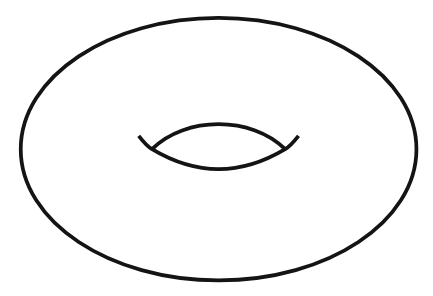
\includegraphics[width=0.3\textwidth]{../Lectures/Figures/torus_1.png}
    }
    \subfloat[]{
        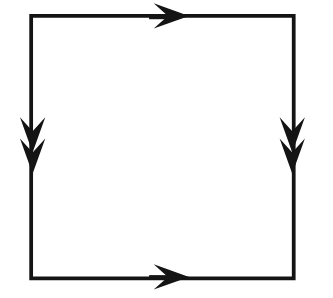
\includegraphics[width=0.3\textwidth]{../Lectures/Figures/torus_2.png}
    }
    \caption{Two Riemannian metrics on torus.}
\end{figure}
\subsection{Existence of a Riemannian Metric}
The local diffeomorphism $\phi$ defines a Riemannian metric on 
a coordinate chart $(U, x^1,\dots, x^n)$ of $M$ that $x^i=r^i \circ \phi$, 
as
\begin{equation}
    \inner{X}{Y}=\sum_{ij}a^i b^i\inner{\partial_i}{\partial_j}
    =\sum_{ij}a^i b^i,
    \label{eq. induced inner}
\end{equation}
since $\phi_* \partial_j=\frac{\partial}{\partial r^j}$, the induced metric 
is the same as the Euclidean ones.

To obtain a Riemannian metric on $M$, we need to piece together the Riemannian 
metrics on all charts of an atlas of $M$. Here, we use the 
\textbf{partition of the unity} as the standard tools.
\begin{theorem}[Existence of a Riemannian metric]
    There exists a Riemannian metric on every manifold.
\end{theorem}
\begin{proof}
    Let $\{(U_\alpha, \phi_\alpha)\}_{\alpha \in A}$ an atlas of $M$. 
    We have a partition of unity $\{\rho_\alpha\}$ that subcoordinates to 
    open sets $\{U_\alpha\}$. 
    Let $\inner{}{}_\alpha$ the Riemannian metric on $U_\alpha$ as in (\ref{eq. induced inner}), 
    from Proposition~\ref{prop. nonneg combinition of metrics}, we define a metric
    on $T_pM$ at $p$ is 
    \begin{align}
        \inner{}{} = \sum_{\alpha\in A} \rho_\alpha \inner{}{}_\alpha.
        \label{eq. piece together metric}
    \end{align}
    Since $U_p$ intersects finite number of $U_\alpha$, (\ref{eq. piece together metric}) is
    a finite sum.
    Since $\rho_\alpha$ and $\inner{}{}_\alpha$ are both smooth, for any $C^\infty$
    vector fields $X, Y$,
    $\sum_{\alpha\in A} \rho_\alpha \inner{X}{Y}_\alpha$ 
    is a finite sum of smooth functions at arbitary $p$
     (By Definition~\ref{def. Riemannian metric}). 
     So $\sum_{\alpha\in A} \rho_\alpha \inner{}{}_\alpha$ is a Riemannian metric on $M$.
\end{proof}

\problemsection{Problems}
\begin{problem}
    Suppose $(M, \inner{}{})$ is a Riemannian manifold. Show that two $C^\infty$ vector fields
    $X,Y \in \mathfrak{X}(M)$ are equal if and only if $\inner{X}{Z}=\inner{Y}{Z}$ for all
    $C^\infty$ vector fields $Z\in\mathfrak{X}(M)$.
\end{problem}